% Artigo WiP (Work in Progress) para o ICIT 2027, no modelo de conferência do IEEE.
% Limite: 4 páginas, já contando figuras e referências. Submissão: 3/11/2026 (prazo final).
% A bibliografia vem de ../referencial/references.bib (não duplicar).
% Os dados das Figs. 3 e 4 vêm de tep-lab/data/experiment_82 e experiment_89 (ver dados/).
\documentclass[conference]{IEEEtran}
\IEEEoverridecommandlockouts

\usepackage[T1]{fontenc}
\usepackage[utf8]{inputenc}
\usepackage{cite}
\usepackage{amsmath,amssymb,amsfonts}
\usepackage{graphicx}
\usepackage{booktabs}
\usepackage{array}
\usepackage{url}
\usepackage{tikz}
\usetikzlibrary{arrows.meta}
\usepackage{pgfplots}
\pgfplotsset{compat=1.18}
\usepgfplotslibrary{groupplots}

\begin{document}

\title{What Must Kubernetes-Based Plant Supervision Demonstrate?\\
Lessons from a First Implementation}

\author{
\IEEEauthorblockN{Matheus Corteletti Delfino}
\IEEEauthorblockA{\textit{Control and Automation Engineering} \\
\textit{Instituto Federal do Espírito Santo (Ifes)}\\
Serra, ES, Brazil \\
matheus.corteletti.del@gmail.com}
\and
\IEEEauthorblockN{Rafael Emerick Zape de Oliveira}
\IEEEauthorblockA{\textit{Control and Automation Engineering} \\
\textit{Instituto Federal do Espírito Santo (Ifes)}\\
Serra, ES, Brazil \\
rafael.emerick@ifes.edu.br}
}

\maketitle

\begin{abstract}
Kubernetes keeps software systems close to a declared desired state, and recent work uses it to run industrial control software. This work in progress asks a different question: what must an implementation demonstrate before one can say that a process plant is under Kubernetes-based supervision? We report our experience with this question. We built a simulation of the Tennessee Eastman Process Benchmark that publishes its signals over OPC~UA, a historian, and custom Kubernetes resources with a controller that evaluates the plant against a declared policy, and we ran them through a feed loss and a slow drift. The controller flagged the feed loss 1.15~h of process time after it occurred. In the drift, cost fell 37\% in 30~h while the plant moved toward shutdown, and the non-compliant verdict came from a declared level limit, 2~h before the shutdown. From this experience we draw a first draft of requirements for such a layer, which our implementation meets only in part. The work in progress is to refine this draft and check it with a new round of runs.
\end{abstract}

\begin{IEEEkeywords}
Kubernetes, supervisory control, process automation, Industry 4.0, OPC UA, Tennessee Eastman Process
\end{IEEEkeywords}

\section{Introduction}

Process plants are operated in layers \cite{Skogestad2004}. Controllers keep variables such as levels and pressures at their setpoints, and a supervisory layer chooses those setpoints and checks whether the plant does what was decided. In the enterprise-control hierarchy of IEC~62264 \cite{IEC62264Std}, this supervision sits between the control systems and the business systems. In practice, the engineers who know how to improve a plant often work on data exported from the historian and analyzed offline.

Software engineering faces a similar problem in distributed systems, and Kubernetes addresses it with a declarative interface: the user declares the desired state, and controllers continuously compare it with the observed state \cite{Burns2016}. This suggested to us a supervisory layer in which the operating policy of a plant is a declared resource and a controller evaluates the plant against it. An operating change then becomes declared, versioned and recorded.

We built such a layer, in which a Kubernetes controller follows a simulated plant, reached over OPC~UA, against a declared policy. The arrangement worked from end to end, but this did not answer whether the plant was supervised. An information security standard such as ISO/IEC~27001 \cite{ISO27001} requires an organization to show that certain processes exist, regardless of the tools it uses. We came to ask the same about our work: what must an implementation demonstrate before one can say that a plant is under Kubernetes-based supervision? This paper reports what we built, what happened when we ran it, and the first draft of requirements that came out of it. We started without a specification, and the draft is a result of the experience, not a standard.

\section{Related Work}

Kubernetes has reached industrial automation mainly as infrastructure for control software. Johansson et~al.\ use it to recover failed controllers with high availability \cite{Johansson2022}, Mellado and Núñez run a programmable logic controller in containers \cite{Mellado2022}, and Koziolek and Burger use a purpose-built Kubernetes operator to update virtual controllers without halting production \cite{Koziolek2022}. In these cases, Kubernetes manages the software that controls the process, not the decisions about how the process should operate.

Two industrial initiatives are closer in intent. The NAMUR Open Architecture (NOA) adds a separate communication path that makes production data available for monitoring and optimization, with no impact on the automation system \cite{NE175}. O-PAS defines conformance profiles for interoperable process automation products, verified by independent laboratories \cite{OPAS}. Our layer shares the separation of NOA, and our draft shares with O-PAS the idea of claims against a specification, but it concerns supervisory behavior and, at this stage, asks for evidence rather than a test suite. These works do not say what a Kubernetes-based supervisory layer must demonstrate.

\section{Kubernetes in Brief}

Kubernetes stores the desired state of a system as objects called \textit{resources}. Programs called \textit{controllers} watch these objects, compare them with what they observe and act on the difference, in a loop called \textit{reconciliation} \cite{Burns2016}. Three concepts allow this mechanism to be extended \cite{K8sOperator}:
\begin{itemize}
\item A \textit{custom resource definition} (CRD) registers a new type of resource in the Kubernetes API, with its name, fields and validation rules. It has no behavior of its own.
\item A \textit{custom resource} is one object of that type, usually written as a text file, the \textit{descriptor}.
\item A \textit{custom controller} is the program that gives the type its behavior. The combination of CRDs and a controller is called an \textit{operator}.
\end{itemize}

The standard objects of Kubernetes do not help here: a Pod or a Deployment describes a program and whether it is running, and has no notion of a reactor level, a cost budget or an operating limit. All of them can be healthy while the plant moves toward shutdown, so supervision in Kubernetes requires new resource types and a controller that evaluates them.

\section{What We Built}

We wanted a plant that runs continuously and can be reached like real equipment, so we rewrote the Downs and Vogel model of the Tennessee Eastman Process (TEP) \cite{DOWNS1993} as a program that publishes its signals over OPC~UA. In steady state, it reproduces the published base-case cost (170.63 against 170.61~\$/h), which checks the model at equilibrium but not its dynamics. All the code is open source\footnote{\raggedright\url{https://github.com/Green-Cinnamon-Labs}.\\ Start at the \texttt{spec-tennessee-eastman} repository.} and Fig.~\ref{fig:arch} shows its parts, on a single-node local cluster. A historian keeps the last 15~minutes of signals and serves window statistics and a control loop performance index \cite{Bradu2018}, so Kubernetes never sees raw signals.

We wrote three CRDs without a prior specification, to try the idea. \texttt{CostFunction} declares the operating cost as a sum of terms, \texttt{OperatingPolicy} declares what the plant should comply with (Fig.~\ref{fig:desc}), and \texttt{Plant} links them and holds the verdict. The process engineer writes the descriptor and applies it with \texttt{kubectl apply}. Every 30~s, and whenever the policy is edited, the controller queries the historian and writes in the \texttt{Plant} status a condition for each criterion and a phase, compliant or not. Reconciliation here ends at the verdict: the controller never writes to the plant.

\begin{figure}[t]
\centering
\footnotesize
\begin{verbatim}
kind: OperatingPolicy
metadata: {name: tep-mode1}
spec:
  costFunctionRef: tep-downs-vogel
  windowSeconds: 60
  maxCost: 170.6
  persistenceEvaluations: 3
  targets:
    - {signal: xmeas.stream11.flow_rate,
       value: 22.949, tolerancePercent: 5}
  constraints:
    - {signal: xmeas.reactor.level,
       min: 50, max: 100}
  # ... other targets, limits and control loops
\end{verbatim}
\vspace{-2mm}
\caption{Excerpt of a descriptor: the engineer declares the cost budget, targets and limits, and how many bad evaluations in a row change the verdict.}
\label{fig:desc}
\end{figure}

\begin{figure}[t]
\centering
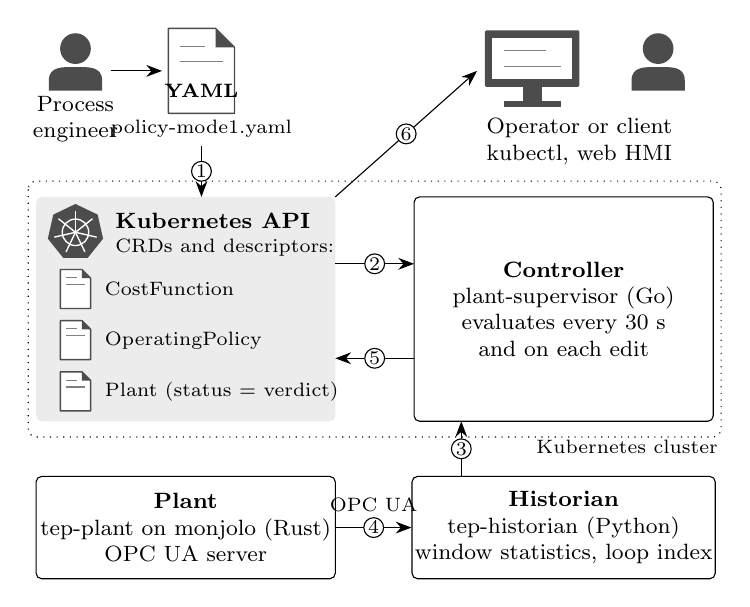
\begin{tikzpicture}[x=1mm,y=1mm,
  >={Stealth[length=2mm]},
  box/.style={draw, rounded corners=2pt, align=center, font=\footnotesize, inner sep=1pt},
  n/.style={circle, draw, fill=white, inner sep=0.4pt, font=\scriptsize},
  lbl/.style={align=center, font=\scriptsize, inner sep=0.5pt},
  person/.pic={
    \fill[black!70] (0,4.1) circle (1.5);
    \fill[black!70] (-2.6,0) -- (-2.6,1) .. controls (-2.6,2.4) and (-1.2,2.3) .. (0,2.3) .. controls (1.2,2.3) and (2.6,2.4) .. (2.6,1) -- (2.6,0) -- cycle;},
  doc/.pic={
    \filldraw[fill=white, draw=black!70, line width=0.5pt, line join=round] (-3.5,-4.5) -- (-3.5,4.5) -- (1.5,4.5) -- (3.5,2.5) -- (3.5,-4.5) -- cycle;
    \fill[black!70] (1.5,4.5) -- (1.5,2.5) -- (3.5,2.5) -- cycle;
    \draw[black!50, line width=0.4pt] (-2.3,2.6) -- (0.4,2.6) (-2.3,1) -- (2.3,1);},
  screen/.pic={
    \fill[black!70, rounded corners=0.5pt] (-5,-1.7) rectangle (5,4.3);
    \fill[white] (-4.2,-0.9) rectangle (4.2,3.5);
    \fill[black!70] (-1,-3.2) rectangle (1,-1.7);
    \fill[black!70] (-3,-3.8) rectangle (3,-3.2);
    \draw[black!50, line width=0.4pt] (-3,2.2) -- (1.5,2.2) (-3,0.5) -- (3,0.5);},
  wheel/.pic={
    \fill[black!70] (90:3) \foreach \a in {1,...,6} { -- (90+\a*360/7:3) } -- cycle;
    \draw[white, line width=0.5pt] (0,0) circle (1.4);
    \foreach \a in {0,...,6} { \draw[white, line width=0.5pt] (0,0) -- (90+\a*360/7:2.3); }}]
% Pessoas e arquivo
\pic[scale=1.3] at (6,-8) {person};
\node[lbl, anchor=north, font=\footnotesize] at (6,-8.5) {Process\\ engineer};
\draw[->] (10.5,-5.5) -- (17,-5.5);
\pic[scale=1.2] at (22,-5.5) {doc};
\node[font=\scriptsize\bfseries, inner sep=0] at (22,-8) {YAML};
\node[lbl, anchor=north] at (22,-11.5) {policy-mode1.yaml};
\pic[scale=1.2] at (64,-5.5) {screen};
\pic[scale=1.3] at (80,-8) {person};
\node[lbl, anchor=north, font=\footnotesize] at (70,-11.3) {Operator or client\\ kubectl, web HMI};
% Cluster
\draw[dotted, rounded corners=3pt] (0,-19.5) rectangle (88,-52);
\node[font=\scriptsize, anchor=north east, inner sep=1pt] at (88,-52) {Kubernetes cluster};
\fill[gray!15, rounded corners=2pt] (1,-21.5) rectangle (39,-50);
\pic[scale=1.2] at (6,-26) {wheel};
\node[anchor=west, font=\footnotesize\bfseries, inner sep=0] at (11,-24.5) {Kubernetes API};
\node[anchor=west, font=\scriptsize, inner sep=0] at (11,-28) {CRDs and descriptors:};
\pic[scale=0.55] at (6,-33.2) {doc};
\node[lbl, anchor=west] at (9.5,-33.2) {CostFunction};
\pic[scale=0.55] at (6,-39.7) {doc};
\node[lbl, anchor=west] at (9.5,-39.7) {OperatingPolicy};
\pic[scale=0.55] at (6,-46.2) {doc};
\node[lbl, anchor=west] at (9.5,-46.2) {Plant (status = verdict)};
\node[box, minimum width=38mm, minimum height=28.5mm] (sup) at (68,-35.75) {\textbf{Controller}\\ plant-supervisor (Go)\\ evaluates every 30~s\\ and on each edit};
% Aplicações fora do cluster
\node[box, minimum width=38mm, minimum height=13mm] (plant) at (20,-63.5) {\textbf{Plant}\\ tep-plant on monjolo (Rust)\\ OPC~UA server};
\node[box, minimum width=38mm, minimum height=13mm] (hist) at (68,-63.5) {\textbf{Historian}\\ tep-historian (Python)\\ window statistics, loop index};
% Setas
\draw[->] (22,-15) -- node[n] {1} (22,-21.5);
\draw[->] (39,-30) -- node[n] {2} (49,-30);
\draw[->] (55,-57) -- node[n] {3} (55,-50);
\draw[->] (plant) -- node[n] {4} node[above=2mm, font=\scriptsize, inner sep=0] {OPC~UA} (hist);
\draw[->] (49,-42) -- node[n] {5} (39,-42);
\draw[->] (39,-21.5) -- node[n] {6} (57,-5.5);
\end{tikzpicture}
\caption{Architecture of the first implementation. Boxes are the applications we developed. 1:~the engineer applies the descriptor. 2:~the controller watches the resources. 3:~it queries aggregates. 4:~the historian reads the plant over OPC~UA. 5:~the controller writes the verdict. 6:~clients read it.}
\label{fig:arch}
\end{figure}

\begin{table*}[t]
\caption{From observations to draft requirements}
\label{tab:draft}
\centering
\footnotesize
\begin{tabular}{@{}>{\raggedright\arraybackslash}p{0.33\textwidth}>{\raggedright\arraybackslash}p{0.37\textwidth}>{\raggedright\arraybackslash}p{0.24\textwidth}@{}}
\toprule
What we observed & An implementation should demonstrate that & Our implementation \\
\midrule
The policy could be edited with the controller running. & The policy is a declared resource, and an edit takes effect within one evaluation. & Built; delay not measured. \\
Verdicts could be read by any client, with their times. & Each verdict is recorded with its time as Kubernetes state. & Met. \\
We designed the controller to withhold a verdict without data. & Missing data produce no verdict, and this is stated. & Built; not exercised in the runs. \\
The controller only reads, and control stays in the plant. & Control and safety stay in the plant controllers, and the plant stays safe if the supervisor fails. & Only reads; supervisor failure not tested. \\
The feed loss was flagged at 1.15~h. & A reference scenario is detected within a limit declared in advance. & No limit declared yet. \\
Criteria come from the literature and are coded by each implementation. & Each criterion is checked against its source on a known scenario before it is trusted. & Not done yet. \\
A new type of criterion required changing code. & It is stated which changes need only a descriptor and which need code. & Thresholds in descriptors; new criteria in code. \\
Cost improved while the level fell, in a variable with no loop. & The policy covers the variables whose loss stops the operation, including trends. & Limits only; no trends. \\
The verdict came 2~h before the shutdown. & The verdict leaves a declared margin to act. & No margin declared yet. \\
What a window covers changes with the plant speed. & Windows and periods state their time base, and judgments do not depend on simulation speed. & Windows in wall-clock time. \\
\bottomrule
\end{tabular}
\end{table*}

\section{What Happened}

All times below are process times. The plant was accelerated, but the 30~s evaluation period is wall-clock time, so each evaluation covered more process time than it would in real operation.

\textit{Normal operation.} We set the cost budget at 170.6~\$/h, the base-case cost, and calibrated the thresholds on a run without disturbance at about ten times real time. Over 41 evaluations, the cost stayed at $166.83 \pm 0.18$~\$/h and all conditions held.

\textit{Feed loss.} At the same speed (about 5~min of process per evaluation), we applied disturbance IDV(6), the loss of feed A (Fig.~\ref{fig:idv6}). The product flow left its target 0.98~h after the disturbance, and the cost exceeded the budget at 1.15~h (about 7~min of wall-clock time), when the phase changed to non-compliant. The verdict followed the physical order of events. We then added a criterion on the setpoint offset, which required changing the historian, the CRD and the controller, not only the policy. In a repeated run, the levels crossed the declared offset at 0.84~h and the loop condition turned false at 1.00~h.

\begin{figure}[t]
\centering
\begin{tikzpicture}
\begin{groupplot}[
  group style={group size=1 by 2, vertical sep=3mm, x descriptions at=edge bottom},
  scale only axis, width=0.68\columnwidth, height=28mm,
  xmin=-1, xmax=2.7, xtick={-1,0,1,2},
  tick label style={font=\scriptsize}, label style={font=\footnotesize},
  ylabel style={yshift=-1mm}, xlabel style={yshift=1mm},
  grid=major, grid style={gray!20}, axis line style={gray!70}, tick style={gray!70},
  clip=true]
\nextgroupplot[ylabel={Cost (\$/h)}, ymin=155, ymax=225, ytick={160,180,200,220}]
\fill[gray!20] (axis cs:1.151,155) rectangle (axis cs:2.7,225);
\addplot[black, thick, mark=none] table[x=t, y=cost] {dados/exp25-custo.dat};
\addplot[black, dashed, mark=none] coordinates {(-1,170.6) (2.7,170.6)};
\node[font=\scriptsize, anchor=south west, inner sep=1pt] at (axis cs:-0.95,171) {budget 170.6};
\draw[gray!70] (axis cs:0,155) -- (axis cs:0,225);
\node[font=\scriptsize, anchor=north east, inner sep=1pt] at (axis cs:-0.03,223) {IDV(6) on};
\draw[gray!70] (axis cs:1.53,155) -- (axis cs:1.53,225);
\node[font=\scriptsize, anchor=north west, inner sep=1pt] at (axis cs:1.56,223) {IDV(6) off};
\node[font=\scriptsize, anchor=south west, inner sep=1pt] at (axis cs:1.56,156) {non-compliant};
\nextgroupplot[height=15mm, xlabel={Process time since the disturbance (h)}, ymin=0.5, ymax=3.5, ytick={1,2,3}, grid=none, ytick style={draw=none},
  yticklabels={PolicyCompliant, TargetsMet, CostWithinBudget}]
\fill[gray!20] (axis cs:1.151,0.5) rectangle (axis cs:2.7,3.5);
\fill[gray!55] (axis cs:-0.923,0.65) rectangle (axis cs:1.151,1.35);
\fill[black] (axis cs:1.151,0.65) rectangle (axis cs:2.623,1.35);
\fill[gray!55] (axis cs:-0.923,1.65) rectangle (axis cs:0.984,2.35);
\fill[black] (axis cs:0.984,1.65) rectangle (axis cs:2.623,2.35);
\fill[gray!55] (axis cs:-0.923,2.65) rectangle (axis cs:1.151,3.35);
\fill[black] (axis cs:1.151,2.65) rectangle (axis cs:2.623,3.35);
\end{groupplot}
\end{tikzpicture}
\caption{Feed loss. Cost from the supervisor status and the Kubernetes conditions that changed (gray: true, black: false). The cost first dips, because less feed A leaves in the purge, and keeps rising after the disturbance ends. Shaded: non-compliant phase.}
\label{fig:idv6}
\end{figure}

\textit{Cost that improves while the plant degrades.} The plant had not recovered after the feed loss, so we changed the three control loops from proportional to PI, a plausible design choice that still left the reactor level without a loop, and ran the plant without disturbance at about 56 times real time (about 28~min of process per evaluation). With proportional loops, the same plant converged. With PI, the purge valve closed slowly and the reactor level fell until the reactor pressure crossed the 3000~kPa shutdown limit at 32.9~h (Fig.~\ref{fig:exp27}). The cost fell from 165.9 to 105.3~\$/h in 30~h, because less reactant left in the purge, and the cost condition held in all 70 evaluations. The level crossed the declared 50\% limit at 29.1~h. In Kubernetes, the condition \texttt{ConstraintsSatisfied} turned false at 30.0~h, and the phase turned non-compliant at 30.9~h, after the three bad evaluations required by the policy. Part of this delay comes from the acceleration, but the level had also fallen for about 25~h inside the allowed range: a fixed limit warns when a variable arrives, not when it starts to drift.

\begin{figure}[t]
\centering
\begin{tikzpicture}
\begin{groupplot}[
  group style={group size=1 by 4, vertical sep=3mm, x descriptions at=edge bottom},
  scale only axis, width=0.68\columnwidth, height=28mm,
  xmin=0, xmax=36, xtick={0,5,...,35},
  tick label style={font=\scriptsize}, label style={font=\footnotesize},
  ylabel style={yshift=-1mm}, xlabel style={yshift=1mm},
  grid=major, grid style={gray!20}, axis line style={gray!70}, tick style={gray!70},
  clip=true]
\nextgroupplot[ylabel={Cost (\$/h)}, ymin=40, ymax=190, ytick={50,100,150}]
\fill[gray!20] (axis cs:30.92,40) rectangle (axis cs:36,190);
\addplot[black, thick, mark=none] table[x=t, y=cost] {dados/exp27-custo.dat};
\addplot[black, dashed, mark=none] coordinates {(0,170.6) (36,170.6)};
\node[font=\scriptsize, anchor=south west, inner sep=1pt] at (axis cs:0.5,171) {budget 170.6};
\node[font=\scriptsize, anchor=south east, inner sep=1pt] at (axis cs:30.6,42) {non-compliant $\rightarrow$};
\draw[gray!70] (axis cs:32.9,40) -- (axis cs:32.9,120);
\nextgroupplot[height=20mm, ymin=0.5, ymax=4.5, ytick={1,2,3,4}, grid=none, ytick style={draw=none},
  yticklabels={PolicyCompliant, ConstraintsSatisfied, TargetsMet, CostWithinBudget}]
\fill[gray!20] (axis cs:30.92,0.5) rectangle (axis cs:36,4.5);
\fill[gray!55] (axis cs:0.16,0.65) rectangle (axis cs:30.92,1.35);
\fill[black] (axis cs:30.92,0.65) rectangle (axis cs:32.83,1.35);
\fill[gray!55] (axis cs:0.16,1.65) rectangle (axis cs:29.96,2.35);
\fill[black] (axis cs:29.96,1.65) rectangle (axis cs:32.83,2.35);
\fill[gray!55] (axis cs:0.16,2.65) rectangle (axis cs:32.45,3.35);
\fill[black] (axis cs:32.45,2.65) rectangle (axis cs:32.83,3.35);
\fill[gray!55] (axis cs:0.16,3.65) rectangle (axis cs:32.83,4.35);
\nextgroupplot[ylabel={Reactor level (\%)}, ymin=10, ymax=80, ytick={25,50,75}]
\fill[gray!20] (axis cs:30.92,10) rectangle (axis cs:36,80);
\addplot[black, thick, mark=none] table[x=t, y=level] {dados/exp27-nivel.dat};
\addplot[black, dashed, mark=none] coordinates {(0,50) (36,50)};
\node[font=\scriptsize, anchor=north west, inner sep=1pt] at (axis cs:0.5,49) {declared limit 50};
\draw[gray!70] (axis cs:32.9,10) -- (axis cs:32.9,80);
\node[font=\scriptsize, anchor=east, inner sep=1pt] at (axis cs:32.8,18) {shutdown};
\nextgroupplot[ylabel={Loop index}, xlabel={Process time (h)}, ymin=0, ymax=1.3, ytick={0,0.5,1},
  legend style={at={(axis cs:18,1.28)}, anchor=north, font=\scriptsize, legend columns=3, draw=none, fill=none, inner sep=1pt, /tikz/every even column/.append style={column sep=2pt}}]
\fill[gray!20] (axis cs:30.92,0) rectangle (axis cs:36,1.3);
\addplot[black, thick, mark=none] table[x=t, y=pressure] {dados/exp27-indice.dat};
\addplot[black!70, dashed, mark=none] table[x=t, y=separator] {dados/exp27-indice.dat};
\addplot[black!70, dotted, thick, mark=none] table[x=t, y=stripper] {dados/exp27-indice.dat};
\addplot[gray!70, densely dashdotted, mark=none, forget plot] coordinates {(0,0.5) (36,0.5)};
\node[font=\scriptsize, anchor=north west, inner sep=1pt] at (axis cs:14.5,0.47) {threshold 0.5};
\legend{pressure, separator level, stripper level}
\end{groupplot}
\end{tikzpicture}
\caption{Run with PI loops. From the top: cost from the supervisor status; Kubernetes conditions (gray: true, black: false); reactor level from the historian; predictability index on the scale of its source, computed offline from the recordings. Shaded: non-compliant phase.}
\label{fig:exp27}
\end{figure}

\textit{Predictability index.} The bottom panel of Fig.~\ref{fig:exp27} shows the index of Bradu et~al.\ \cite{Bradu2018}: the more of the error of a control loop an autoregressive model predicts, the lower the index, which suggests that the loop can improve. We computed it offline from the recordings, with the controller's persistence and a threshold of 0.5 calibrated on the normal run. These values are not the loop condition recorded by the controller, which we do not show, and the phase does not depend on them. The index flagged the loops from 2.1 to 12.6~h, mostly the pressure loop, and again at the last evaluation, but not during the fall of the level, a variable with no loop. It also flagged 4\% of the evaluations in the converging run, against 33\% here. At this speed, its 300~s wall-clock window covers about 4.7~h of process, so we take these values as preliminary.

\section{From the Lessons to a Draft Specification}
\label{sec:draft}

Table~\ref{tab:draft} turns what we observed into draft requirements, and shows where our implementation stands. Like ISO/IEC~27001 \cite{ISO27001}, which states requirements and is checked by audit, the draft does not fix numerical limits or prescribe tests, because they depend on the plant and on the criteria chosen. The implementation declares its thresholds in advance and presents evidence, and the decision comes from comparing the two. A scenario test is one way to produce evidence.

\section{Ongoing Work}

The draft in Table~\ref{tab:draft} covers only observation, because this is all we have tried. It is the main work in progress: we will make its requirements precise, adjust our implementation to them, declare the thresholds in advance, and carry out a new round of runs, whose data we intend to present. In that round, the controller will judge the loops with the index on the scale of its source and a recalibrated threshold.

\textit{Acting on the plant.} When the supervisor only observes, a correct verdict may come too late to act on. We are designing the supervisor to treat a setpoint change as Kubernetes treats a software deployment: applied in steps, verified, tested first on a digital twin, and rolled back if a declared condition fails. We expect this to add requirements to the draft.

\textit{Second plant and other groups.} The next plant is a didactic level process at Ifes, where a PID in the plant controller drives a pump and the setpoint is exposed through an OPC server. Its model will first be written in \texttt{monjolo}; experiments on the physical plant depend on access and authorization, which have not been confirmed yet. We also plan to simplify the stack, with a Python interface for plant models, a historian template and a single-command cluster setup. The target is concrete: a second group brings its own plant under supervision with no changes to the controller code, only new descriptors, and presents its evidence.

\section{Conclusion}

We asked what an implementation must demonstrate before a plant can be said to be under Kubernetes-based supervision, and we approached the question by building one. We learned four things. The arrangement works from end to end: a Kubernetes controller followed a simulated plant, reached over OPC~UA, against a declared policy, and within Kubernetes this requires CRDs and a controller, because the standard objects know nothing of the process. A detection delay can only be judged against a limit declared in advance. A policy must watch more than cost, which can improve while the plant degrades. And observation alone may leave little time to act.

These lessons became a first draft of requirements, which our implementation meets only in part. The work that remains is to make the draft precise and check it with a new round of runs, to test the layer in real time, on a physical plant and on a multi-node cluster, to let the supervisor act on the plant, and to have a second group bring its own plant under supervision.

\section*{Acknowledgment}

The text of all sections and the code of Figs.~\ref{fig:arch} to~\ref{fig:exp27} were drafted with Claude Opus 5.5 (Anthropic), through Claude Code, from the authors' thesis, software and notes. The authors reviewed the content and are responsible for it.

\bibliographystyle{IEEEtran}
\bibliography{../referencial/references}

\end{document}
